\section{数学分析}{
\subsection{映射与函数}{

\subsubsection{映射}{
    映射指的是集合之间的一种对应关系.

    定义 : $X,Y$是两集合,按照某个规则$f$,对于任一的$x \in X$,有唯一的$y \in Y$与之对应,则称$f$是$X$到$Y$的一个映射.

    记为 : $f: X \to Y$,即 : $x \mapsto y = \defFunction{x}$

    称呼 :

    \begin{itemize}
        \item $y$ : 在映射$f$下,x的像.
        \item $x$ : 在映射$f$下,y的\textcolor{red}{一个}逆像.
        \item $X$ : $f$的定义域,记为$X = D_f$.
        \item $Y$ : $f$的值域,记为$R_f \subset Y$,具体的来说,$R_f = \set{y | y \in Y \land \exists x(y = f(x) \land x \in X)}$
    \end{itemize}

    举例 : 设$X$是平面上三角形的全体,$Y$是平面上圆的全体,构造一个映射$f$,表示(y 是 x 的外接圆),记为 : $$
        f : \underset{x \mapsto y}{X \to Y}
    $$
}%映射结尾

\subsubsection{映射的基本要素}{
    \begin{itemize}
        \item $X = D_f$,定义域.
        \item $Y$,限制值域的范围.
        \item $f$,需要保证像的唯一性.
    \end{itemize}

    这说明了两点 : \begin{enumerate}
        \item {
              映射的像是唯一的,举例 :

              设$X = \mathRealNumberCollection^+ = \set{x | x \in R \land x > 0}$,假设存在映射$f : \underset{x \mapsto y}{X \to Y}(y^2 = x)$,此时$Y = \mathRealNumberCollection$,那么假设$x = 4,y = \pm 2$.这个映射就无法保证像的唯一性.换句话说,这个$f$并不是个映射.

              但是可以稍作改造:对$Y = \mathRealNumberCollection$做限制,令$Y = R^-$,此时 : $$
                  \mapsToWithSubText{f}{X \to Y}{x \mapsto y}(y^2 = x)
              $$
              就构成了一个映射
              }
        \item {
              映射不要求逆向唯一.
              }
    \end{enumerate}
}%映射的基本要素结尾

\subsubsection{映射的分类}{
    \begin{itemize}
        \item {
              单射 :

              $f$是$X$到$Y$的一个映射,若逆像也具有唯一性,则称$f$是单射(injection)

              逻辑命题表述 : $x_1 \neq x_2 \Rightarrow y_1 \neq y_2(y_1 = \defFunction{x_1},y_2 = \defFunction{x_2})$

              注 : 单射的值域不一定完全等于$Y$,也可能包含于$Y$,即$R_f \subseteq Y$
              }
        \item {
              满射 : 如果映射的值域完全等于$Y$,即$R_f = Y$,则称为满射(surjection).

              注 : 满射不一定是单射
              }
        \item {
              双射 : 如果$f$又是单射,又是满射,则称$f$为双射(bijection)

              双射又称为一一对应.
              }
    \end{itemize}
}%映射的分类结尾

\subsubsection{逆映射}{
    如果$f : X \to Y$是一个单射,即对任意的$y \in R_f$,有唯一的逆像$x \in X$与$y$对应.

    如果$\mapsToWithSubText{g}{R_f \to X}{y \mapsto x}$是满射($\defFunction{x} = y$)

    那么$g$就称为$f$的逆映射,又记为$f\inverse$

    举例 : $\mapsToWithSubText{y = \sin x}{\mediumBigCase{-\frac{\pi}{2},\frac{\pi}{2}} \to \mediumBigCase{-1,1}}{x \mapsto y = \sin x}$,他的逆映射为 : $$
        \mapsToWithSubText{x = \arcsin y}{\mediumBigCase{-1,1} \to \mediumBigCase{-\frac{\pi}{2},\frac{\pi}{2}}}{y \mapsto x}(\sin x = y)
    $$
}%逆映射结尾

\subsubsection{复合映射}{
    $$
        \mapsToWithSubText{g}{X \to U_1}{x \mapsto u = g(x)}
    $$
    $$
        \mapsToWithSubText{f}{U_2 \to Y}{u \mapsto y = f(u)}
    $$

    这两个映射若是要复合在一起,那么就得满足 : $R_g \subset U_2 = D_f$.即 : $g$的值域在$f$的定义域中,才能构造出复合映射.

    称为$f$与$g$的复合映射.

    例 : 设$X = Y = U_1 = U_2 = \mathRealNumberCollection$ :
    $$
        \mapsToWithSubText{g}{x \to U_1}{x \mapsto u = \sin x}
    $$
    $$
        \mapsToWithSubText{f}{U_2 \to Y}{u \mapsto y = \frac{u}{1 + u^2}}
    $$
    由于$R_g = \mediumBigCase{-1,1} \subset D_f$,所以 : $$
        \mapsToWithSubText{f \cdot g}{X \to Y}{x \mapsto y = \frac{\sin x}{1 + \sin x}}
    $$
}%复合映射结尾

\subsubsection{函数}{
    函数是映射的特殊情况.

    有映射 : $$
        \mapsToWithSubText{f}{X \to Y}{x \mapsto y = \defFunction{x}}
    $$
    如果$X \subset \mathRealNumberCollection,Y = \mathRealNumberCollection$,即如果两者都是实数构成的集合,那么就称$f$为一元实函数(简称函数).

    如果$X$是卡氏积(笛卡尔乘积集合),那么就是多元实函数.

    对函数来说,映射可以简写为 : $$
        y = \defFunction{x},x \in X\ (X = D_f)
    $$
    其中$x$也称为自变量,$y$称为因变量,函数也反映了因变量与自变量变化的一种因果关系.
}%函数结尾

\subsubsection{基本初等函数}{
    以下几种函数被称为基本初等函数 :

    \begin{enumerate}
        \item 常数函数 : $y = \mathConstant$
        \item 幂函数 : $y = x^\alpha\ (\alpha \in \mathRealNumberCollection)$
        \item 指数函数 : $y = a^x\ (a > 0 \land a \neq 1)$
        \item 对数函数 : $y = \log_ax\ (a > 0 \land a \neq 1)$
        \item 三角函数 : $y = \sin x,\cos x,\tan x,\cot x...$
        \item 反三角函数 : $y = \arcsin x,\arccos x,\arctan x...$
    \end{enumerate}
}%基本初等函数结尾

\subsubsection{初等函数}{
    初等函数是由基本初等函数经过有限次四则运算与复合运算所产生的函数.

    例如 : $$
        y = ax^2 + bx + c
    $$
}%初等函数结尾

\subsubsection{自然定义域}{
自然定义域是指函数中自变量的最大取值范围.

如果函数不注明定义域,则默认定义域为他的自然定义域.

例 : 求$y = x + \frac{1}{x}$的自然定义域 : $$
    D = (-\infty,0) \unionSet (0,+\infty),\ R = (-\infty,-2] \unionSet [2,+\infty)
$$

方法不说了...难以描述.
}%自然定义域结尾

\subsubsection{函数的表示}{
    \begin{itemize}
        \item 显式表示 : $y = \defFunction{x}$
        \item {
              分段表示 :

              $A \intersectionSet B = \emptyset$,现有$\varphi(x)$定义于$A$上,$\psi(x)$定义于$B$上,构造函数$\defFunction{x}$ : $$
                  \defFunction{x} = \begin{cases}
                      \varphi(x)\qquad x \in A \\
                      \psi(x)\qquad x \in B
                  \end{cases}
              $$

              这样的表示称为函数的分段表示.
              }
        \item {
              隐函数表示(函数的隐式表示) : $F(x,y) = 0$

              也就是说没有写成$y = F(x)$的形式,而是写成了方程的形式,式中$y$与$x$的变化关系并没有写出,而是写在方程中.

              例如 : $$
                  x^2 + y^2 = R^2\mbox{或者}x^2 + y^2 - R^2 = 0
              $$

              发现对任意的$x \in (-\mathRealNumberCollection,+\mathRealNumberCollection)$,都有两个$y$与之对应.

              这并不意味着这个函数关系无法讨论,只需要对$y$做限制,比如要求$y \geq 0$,这样一来对于给定的$y$,就有唯一确定的$x$,由此就构成了函数关系.

              需要注意的是并不是所有的隐函数都可以写出显式表达的形式,比如Kepler方程 : $$
                  y = x + \varepsilon \sin y
              $$

              这个方程描述了行星绕太阳运行的轨迹的规律,轨迹是个椭圆.其中$\varepsilon$是这个椭圆的离心,$x$与时间有关,$y$与行星的位置有关.
              }
        \item {
              参数表示 :

              当$x$与$y$的关系不方便表示的时候可以考虑引进参数$t$($t$只是个字符),如果$x$和$y$可以表示成$t$的函数 : $$
                  \begin{cases}
                      x = x(t) \\
                      y = y(t)
                  \end{cases},\ t \in [a,b]
              $$

              这样就间接的反映了变量$y$与$x$之间的参数表示,称为函数的参数表示.

              他是这么表示的 : 有两个集合 : $$
                  X = \set{x | x = x(t),t \in [a,b]},\ Y = \set{y | y = y(t),t \in [a,b]}
              $$

              那么函数关系$f$就是一个映射 : $$
                  \mapsToWithSubText{f}{X \to Y}{x = x(t) \mapsto y = y(t)}
              $$
              }
    \end{itemize}
}%函数的表示结尾

\subsubsection{函数的简单性质}{
    \begin{enumerate}
        \item {
              有界性 : 对于$y = \defFunction{x},x \in D$ :

              如果存在$m < M$,使得$m \leq \defFunction{x} \leq M,x \in D$,则称$\defFunction{x}$有界,$m$称为下界,$M$称为上界.

              等价定义 : 存在$X > 0$(此$X$不是集合),使得$\absoluteValue{\defFunction{x}} \leq X,x \in D$

              需要注意的是 : 如果函数有界,那么上下界是不唯一的.
              }
        \item {
              单调性 : 对于$y = \defFunction{x},x \in D$ :

              若对于任意的$x_1,x_2 \in D,x_1 < x_2 \Leftrightarrow \defFunction{x_1} \leq \defFunction{x_2}$,则称函数$f$在$D$单调增加.如果$\leq$可以换成$<$,则称为严格单调增加.

              记为 : $$
                  f\uparrow(f\mbox{严格}\uparrow)
              $$

              类似的,将不等号的箭头方向改变,也有单调减少和严格单调减少,记为 : $$
                  f\downarrow(f\mbox{严格}\downarrow)
              $$
              }
              \item {
                  
              }
    \end{enumerate}
}%函数的简单性质结尾

\subsubsection{一些特殊的函数}{
    \begin{itemize}
        \item {
              符号函数 :

              符号函数(Sign function,简称sgn)是一个逻辑函数,用以判断实数的正负号.为避免和英文读音相似的正弦函数(sine)混淆,它亦称为Signum function.其定义为 : $$
                  sgn(x) = \begin{cases}
                      -1\qquad x < 0 \\
                      0\qquad x = 0  \\
                      1\qquad x > 0
                  \end{cases}
              $$

              \functionTabular{$D = (-\infty,+\infty)$}{$R = sgn(x) = \set{-1,0,1}$}{奇函数}

              图像为 :

              \begin{center}
                  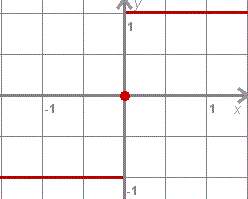
\includegraphics[scale=0.5]{resources/Signum_function.png}
              \end{center}
              }
        \item {
              整数部分函数(下取整函数) :$$
                  y = [x]
              $$

              在数学和计算机科学中,取整函数是一类将实数映射到相近的整数的函数.

              常用的取整函数有两个,分别是下取整函数和上取整函数.

              下取整函数即为取底符号,在数学中一般记作$[x]$或者$E(x)$,在计算机科学中一般记作$floor(x)$,表示不超过$x$的整数中最大的一个 : $$
                  [x] = \min\set{n \in \mathIntegerCollection | x \leq n}
              $$

              \functionTabular{$D = (-\infty,+\infty)$}{$R = [X] = \mathIntegerCollection$}{N/A}

              图像为 :

              \begin{center}
                  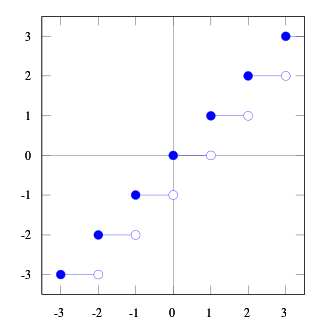
\includegraphics[scale=0.5]{resources/Floor_function.png}
              \end{center}

              下取整函数的符号用方括号$[x]$表示,称作高斯符号.
              }
        \item {
              小数部分函数(分数部分函数) : $$
                  y = (x) = x - [x]
              $$

              小数部分函数(decimal part function)亦称分数部分函数,是一种特殊的数论函数.$x$的小数部分记为${x}$,读作$x$的小数部分(或分数部分).小数部分函数被定义为${x}=x-[x]$,其中$[x]$是整数函数.$\{x\}$只能是0或正的纯小数,即$\{x\}$满足$0≤\{x\}<1$

              \functionTabular{$D = (-\infty,+\infty)$}{$R = \{X\} = (0,1)$}{N/A}

              图像为 :

              \begin{center}
                  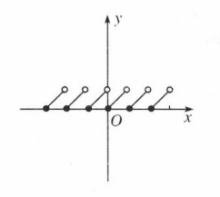
\includegraphics[]{resources/DecimalPartFunction.png}
              \end{center}
              }
    \end{itemize}
}%一些特殊的函数结尾

}%映射与函数结尾

}%数学分析结尾